\chapter{Scientific Workflow Partitioning in a Multisite Cloud} \label{SWPMC}

As the scale of the data increases, SWfMSs need to support SWf execution in High Performance Computing (HPC) environments. Because of various benefits, cloud emerges as an appropriate infrastructure for SWf execution. 
However, it is difficult to execute some SWfs at a cloud site because of geographical distribution of scientists, data and computing resources. Therefore, a SWf often needs to be partitioned and executed in a multisite environment. 
This chapter proposes a non-intrusive approach to execute SWfs in a multisite cloud with three SWf partitioning techniques. This chapter is based on \cite{Liu2014}.

Section \ref{sec:SWEMCSM} introduces our system model based on an adaptation of Chiron for multisite cloud. Then, Section \ref{sec:UCBuzz} presents the Buzz SWf we use for experimentation. Section \ref{sec:WPT} details our three SWf partitioning techniques and Section \ref{sec:SWEMCVal} presents our experimental validation in Microsoft Azure. 
The experimental validation used an adaptation of Chiron SWfMS for Microsoft Azure multisite cloud. The experiment results reveal the efficiency of our partitioning techniques, and their superiority in different environments.

\section{Overview of the Proposal and Motivations}

Scientific experiments generally contain multiple computational activities to process experimental data and these activities are related by data or control dependencies. SWfs enable scientists to model these data processing activities together to be automatically executed. In a SWf, one activity may consist of several executable tasks for different parts of experimental data during SWf execution. SWfs exploit SWfMSs to manage SWf representation, execution and data sets in various computing environments. SWfMSs may exploit High Performance Computing (HPC) to execute SWfs within reasonable time. The HPC environment may be provided by a cluster, grid or cloud. Cloud computing, which promises virtually infinite resources, scalable services, stable service quality and flexible payment policies, has recently become a viable solution for SWf execution. 

In general, one cloud site is sufficient for executing one user application. However, in the case of SWfs, some important restrictions may force their execution in a multisite cloud, \textit{i.e.} a cloud with multiple distributed data centers, each being explicitly accessible to cloud users. For instance, some activities need to be executed at a cloud site trusted by the scientists for SWf monitoring without malicious attack, \textit{i.e.} scientist security restriction; some activities need to be moved to another cloud site because of stored big input data at that site and the cost of transferring this big data to another site is very high, \textit{i.e.} data transfer restriction;
some activities have to be executed at a site where more computing resources are available, \textit{i.e.} computing capacity restriction; some other activities may invoke special programs (instruction data), which are located at a specific cloud site and cannot be moved to another site because of proprietary reasons, \textit{i.e.} proprietary restriction. The configuration data, which includes SWf representation files or SWf parameters, can be located at one site or distributed at different sites. In this situation, multisite cloud is appealing for data-intensive SWfs.

For a given application, a multisite cloud configuration, which is the configuration of Virtual Machines (VMs) at each site, can be homogeneous, with homogeneous computing capacity at each site, \textit{e.g.} $8$ VMs at sites $1$ and $2$, or heterogeneous, \textit{e.g.} $8$ VMs at site $1$ and $2$ VMs at site $2$. The homogeneous configuration is obviously easier to deal with in terms of SWf partitioning and execution. However, even the homogeneous configuration makes it difficult to reproduce experiments as the allocation of VMs to real resources is typically controlled at runtime by the
cloud provider. For instance, at time $t_1$, one VM may be allocated to a processor that is already very busy (\textit{e.g.} running $16$ other VMs) while at time $t_2$, the same VM may be allocated to an underloaded processor (\textit{e.g.} running $2$ other VMs).

In order to execute SWfs in a multisite cloud environment, a SWfMS can generate a Workflow Execution Plan (WEP) for SWf execution. Similar to the concept of Query Execution Plan (QEP) in distributed database systems \cite{Ozsu2011}, the WEP is a program that captures optimization decisions and execution directives, typically the result of compiling and optimizing a SWf. 
Since the multiple sites are interconnected but share nothing, the WEP includes a SWf partitioning result, which is the decision of partitioning a SWf into SWf fragments for independent execution.
A SWf fragment (or fragment for short) can be defined as a subset of activities and data dependencies of the original SWf (see \cite{Ogasawara2011} for a formal definition). In order to execute a fragment within reasonable time at one site, the WEP generally contains a SWf parallelization plan, which parallelizes SWf execution.

We formulate the problems addressed in this chapter as follows. A SWf \textit{$W$} = \{\textit{$V$},\textit{$E$}\} consists of a set of activities \textit{$V$} and a set of dependencies \textit{$E$}. A multisite cloud \textit{$MS$} = \{\textit{$S_{1}$}, \textit{$S_{2}$}, ..., \textit{$S_{n}$}\} is composed of multiple cloud sites, each of which has multiple computing nodes and stores its own data (input data, instruction data or configuration data of \textit{$W$}).
The SWf execution time is the entire time to execute a SWf at a given execution environment.
Given a SWf \textit{$W$} and a multisite cloud \textit{$MS$}, the multisite cloud execution problem is how to execute \textit{$W$} in \textit{$MS$} in a way that
reduces execution time while respecting restrictions.

We propose a non-intrusive approach to execute a SWf in a multisite cloud. We propose three partitioning techniques with the consideration of restrictions. We validate our approach with a data-intensive SWf using Chiron \cite{Ogasawara2013} SWfMS in Microsoft Azure \cite{Azure} cloud.
The experiment results reveal that our approach can reduce execution time. Since the occupied computing resources do not change, the reduction of execution time may lead to less lease time, 
which corresponds to less monetary cost.

\section{Related Work}
\label{sec:SWEMCRW}
SWf partitioning and execution in a multisite cloud remains a challenge and little work has been done. Deng \textit{et al.} \cite{Deng2011} adopt a clustering method based on data-data, data-activity and activity-activity dependencies. This method is adapted for SWf structures, but it may have big amount of data to be transferred among fragments. Chen \textit{et al.} \cite{Chen2012} present SWf partitioning based on storage constraints. Since a cloud environment can offer big storage capacity and the VMs can be mounted additional storage resources before or during SWf exeuciton, the storage capacity limitation is not general in a cloud environment. 
In addition, this method do not take data transfer cost and different computing capacity at each site into consideration. Tanaka and Tatebe \cite{Tanaka2012} use a Multi-Constraint Graph Partitioning (MCGP) algorithm \cite{Karypis1998} to partition a SWf. This approach partitions a SWf by minimizing the removed dependency and balancing the activities in each fragment.
However, this approach is appropriate only for homogeneous execution sites.
In this chapter, we propose several partitioning techniques to address data transfer restriction and computing capacity restriction in the multisite cloud. Because of SWf partitioning, distributed provenance data is supported in the multisite cloud. In addition, data compression and file archiving is proposed to accelerate the data transfer between different cloud sites.


\section{System Model}
\label{sec:SWEMCSM}
In this section, we present our system model based on Chiron SWfMS, its adaptation for multisite cloud and a SWf partitioner.

Chiron implements an algebraic approach for data-intensive SWfs proposed by Ogasawara \textit{et al.} \cite{Ogasawara2013}, to perform SWf parallelization and scheduling. This approach associates each activity with an operator, which has a semantic meaning for parallel execution.
Since it models SWf data as relations similar to relational database management systems, 
this approach can optimize the entire SWf parallel execution based on well-founded relational algebra query optimization models \cite{Ogasawara2011}.

The algebraic approach also allows online provenance data to be managed (and stored in a database by Chiron) for SWf activity monitoring \cite{Costa2013}. Provenance data is the metadata that captures the derivation history of a dataset, including the original data sources, intermediate datasets, and the SWf computational steps that were applied to produce this dataset \cite{Costa2013}.

Chiron was initially developed for a one site execution environment as shown in Fig. \ref{fig:f2}-$A$. 
In a one site environment, a database is installed in a master node
and all the computing nodes share storage resources through Network File System.
Chiron achieves activity parallelism, data parallelism and dynamic scheduling for SWf parallelization as explained in Section \ref{sec:SWEMCRW}.
Chiron was modified to gather necessary produced data at the end of SWf execution at one site.

In a multisite cloud environment (see Fig. \ref{fig:f2}-$B$), all the sites have the same configuration as one site environment, \textit{i.e.} a database installed in a master node and shared storage resources, while each site can have different numbers of slave computing nodes. We developped a SWf partitioner to automatically partition a processed SWf representation file into SWf fragment representation files
when the first activity in each fragment is given.
All the activities in a fragment are placed together in the processed SWf representation file.
The SWf partitioner removes the dependencies in the original SWf and generates corresponding configuration files for each fragment.
The execution of the generated fragments should respect the dependencies removed from the original SWf. 
Let us suppose that, in a SWf, activity \textit{$A_{2}$} consumes the output data produced by activity \textit{$A_{1}$}.
If these two activities are allocated to different fragments, 
their data dependencies will be removed from the explicit data dependencies. 
In this case, the fragment that contains activity \textit{$A_{2}$} should be executed after 
the execution of the fragment that contains activity \textit{$A_{1}$}. 

In order to reduce data transfer volume between different sites, we can use data compression and file archiving techniques. Data compression can just reduce the volume of transferred data to reduce transmission time. Through file archiving, we can also transfer the data at a relatively high speed to reduce transmission time. When transferring one file between two sites and the default transfer speed is less than the average transfer speed between two sites, the file transfer is accelerated (accelerating phase) at the beginning and decreased (decreasing phase) at the end. The data transfer rate remains high in the middle (high speed transfer phase).
If we transfer several small files, there will be many accelerating and decreasing phases.
But if we transfer a big file of the same data volume, there will be an accelerating phase and a decreasing phase while the high speed transfer phase will be longer. Therefore, the transmission speed of a big file is higher than that of several small files of the same data volume. In the remainder of the chapter, we note data refining as the combination of file archiving and data compression.


\begin{figure}
\begin{centering}
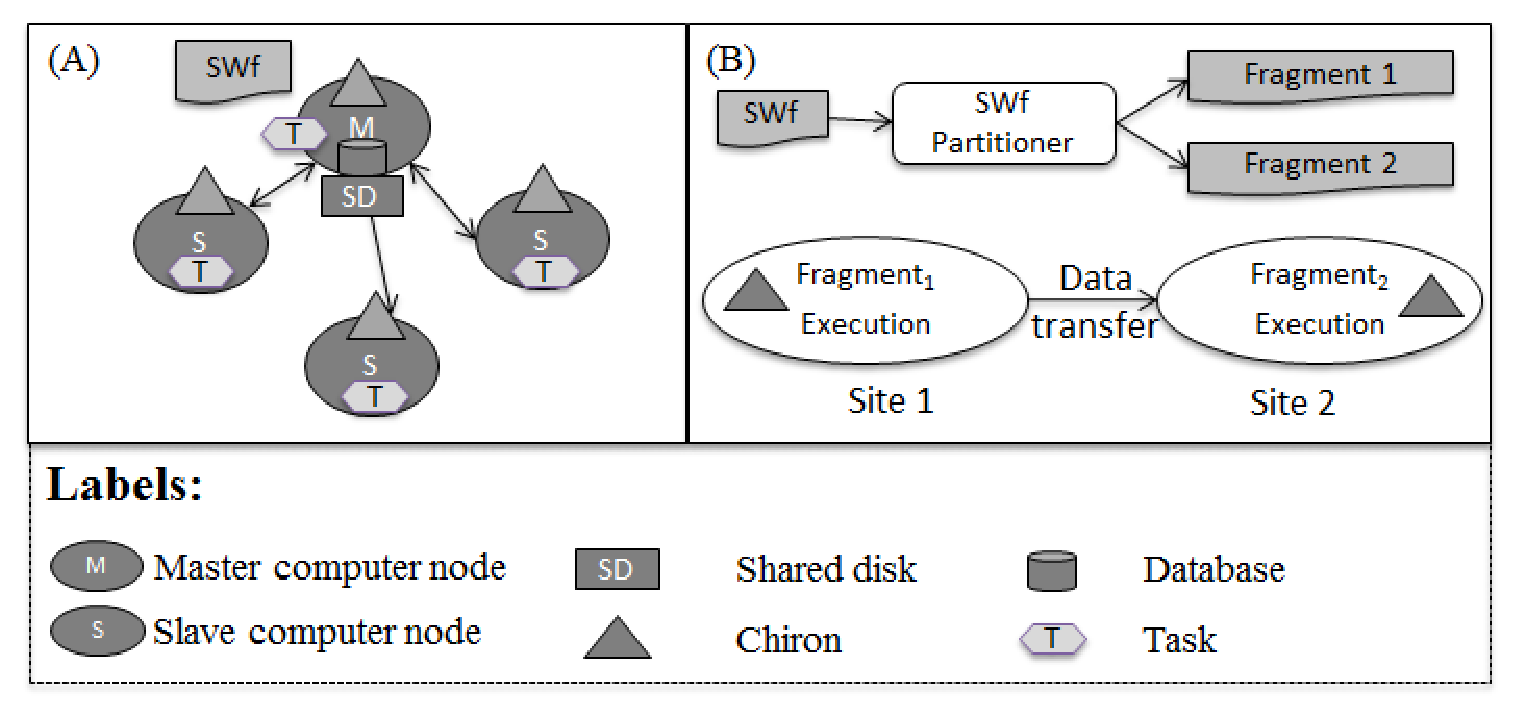
\includegraphics[width=4in]{figures/SF4_fragment.eps}
\par\end{centering}
\caption{\textbf{The architecture of SWf Execution in Chiron. } Fig. $A$ presents SWf execution in one site using Chiron before modification. Fig. $B$ shows the multisite SWf execution using SWf partitioner and modified Chiron.}
\label{fig:f2} 
\end{figure}

\section{Use Case: Buzz Workflow}
\label{sec:UCBuzz}
This section presents Buzz SWf \cite{Dias2013}, a data-intensive SWf, as a use case to illustrate our partitioning techniques. Buzz SWf is modeled and executed using Chiron. Buzz SWf searches for trends and measures correlations in published papers from scientific publications. This SWf uses data collected from bibliography databases such as the DBLP Computer Science Bibliography (DBLP) \cite{dblp} or the U.S. National Institutes of Health's National Library of Medicine (PubMed). 
We used a DBLP 2013 XML file of $1,29$GB as input for Buzz SWf in our experiments.

Buzz SWf has thirteen activities (Fig. \ref{fig:f1-0}). 
Each activity has a specific operator according to the algebraic approach. 
Boxes in the figure represent activities together with the involved algebraic operators. 
\textit{FileSplit} activity is responsible for gathering all scientific publications from bibliography databases. 
\textit{Buzz} activity uses these publications to identify buzzwords (a word or phrase that can become popular for a specific period of time).
\textit{WordReduce} activity organizes these publications according to buzzword and publication year, 
and it also computes occurrences of identified words. 
Furthermore, \textit{YearFilter} activity selects buzzwords that appeared in the publications after $1991$, 
while \textit{BuzzHistory} activity and \textit{FrequencySort} activity create a history for each word and compute its frequency. 
With this information, \textit{HistogramCreator} activity generates some histograms with word frequency varying the year. 
On the other hand, \textit{Top$10$} activity selects ten of the most frequent words in recent years, 
whilst \textit{ZipfFilter} activity selects terms according to a Zipf curve that is specified by word frequency values \cite{Tarapanoff2001}. 
Moreover, \textit{CrossJoin} activity merges results from \textit{Top$10$} activity and \textit{ZipfFilter} activity. 
\textit{Correlate} activity computes correlations between the words from \textit{Top$10$} activity and buzzwords from \textit{ZipfFilter} activity. 
Using these correlations, \textit{TopCorrelations} activity takes the terms that have a correlation greater than a threshold 
and \textit{GatherResults} activity presents these selected words with the histograms. 

\begin{figure}
	\begin{centering}
		\subfigure[\textbf{Buzz SWf.}]{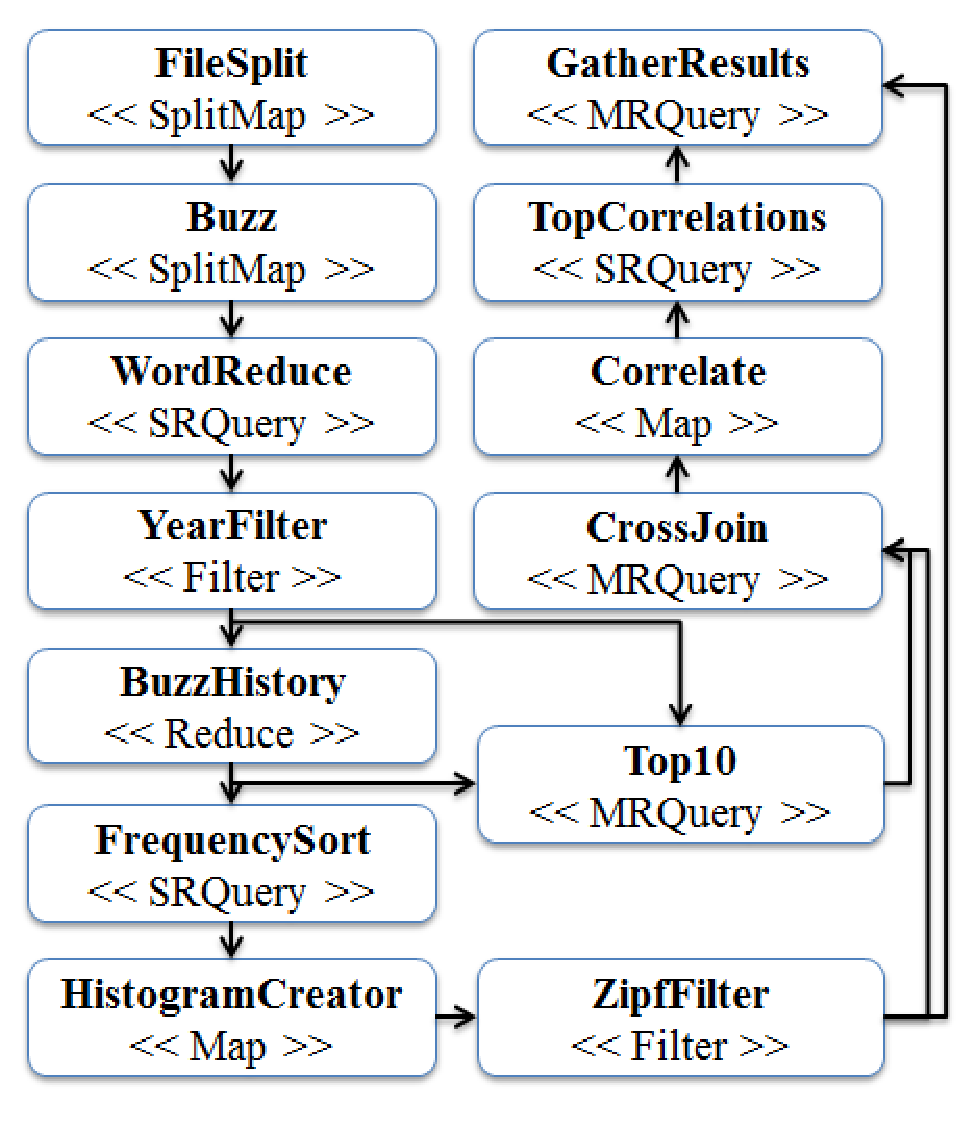
\includegraphics[width=2.3in]{figures/SF0} \label{fig:f1-0}} 
		\subfigure[\textbf{Scientist privacy technique.}]{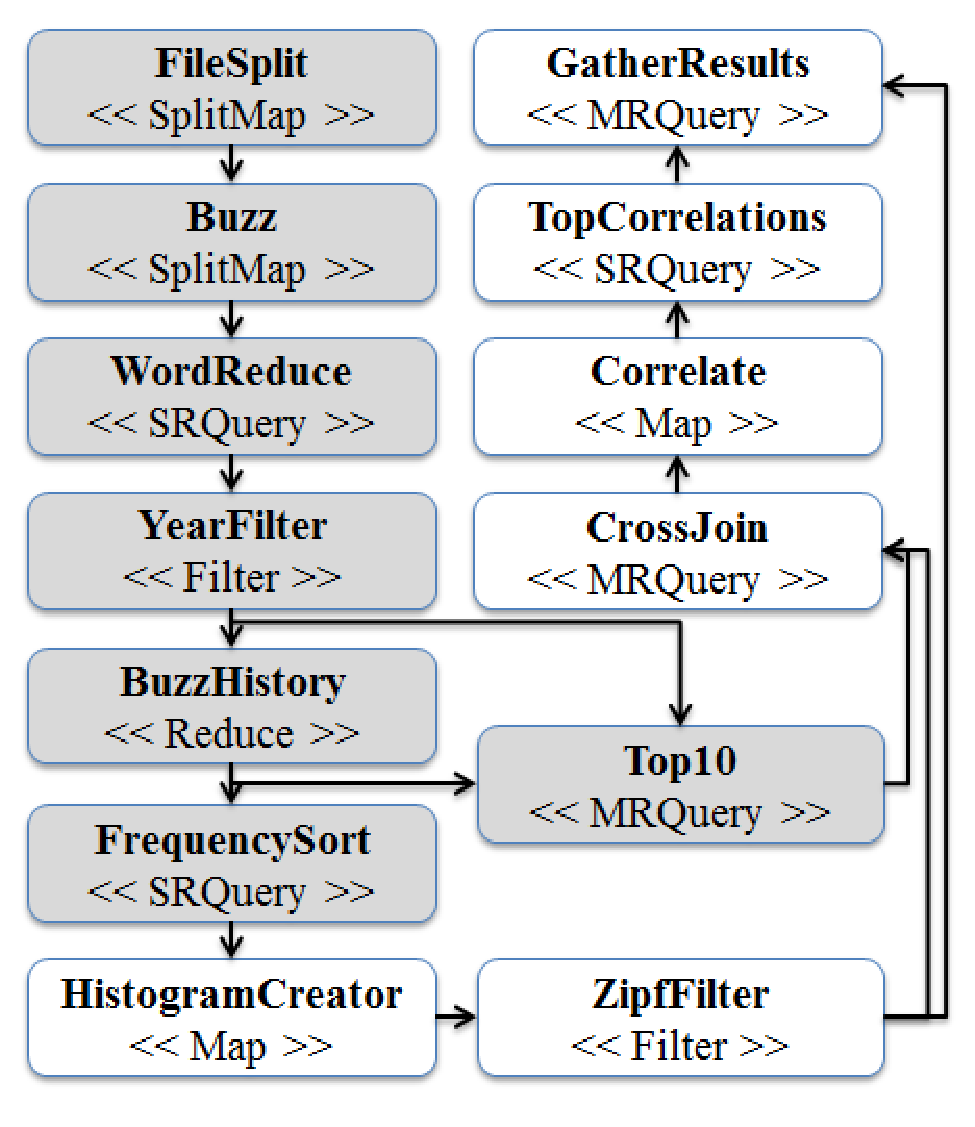
\includegraphics[width=2.3in]{figures/SF1} \label{fig:f1-1}} \\
		\subfigure[\textbf{Data transfer minimization technique.}]{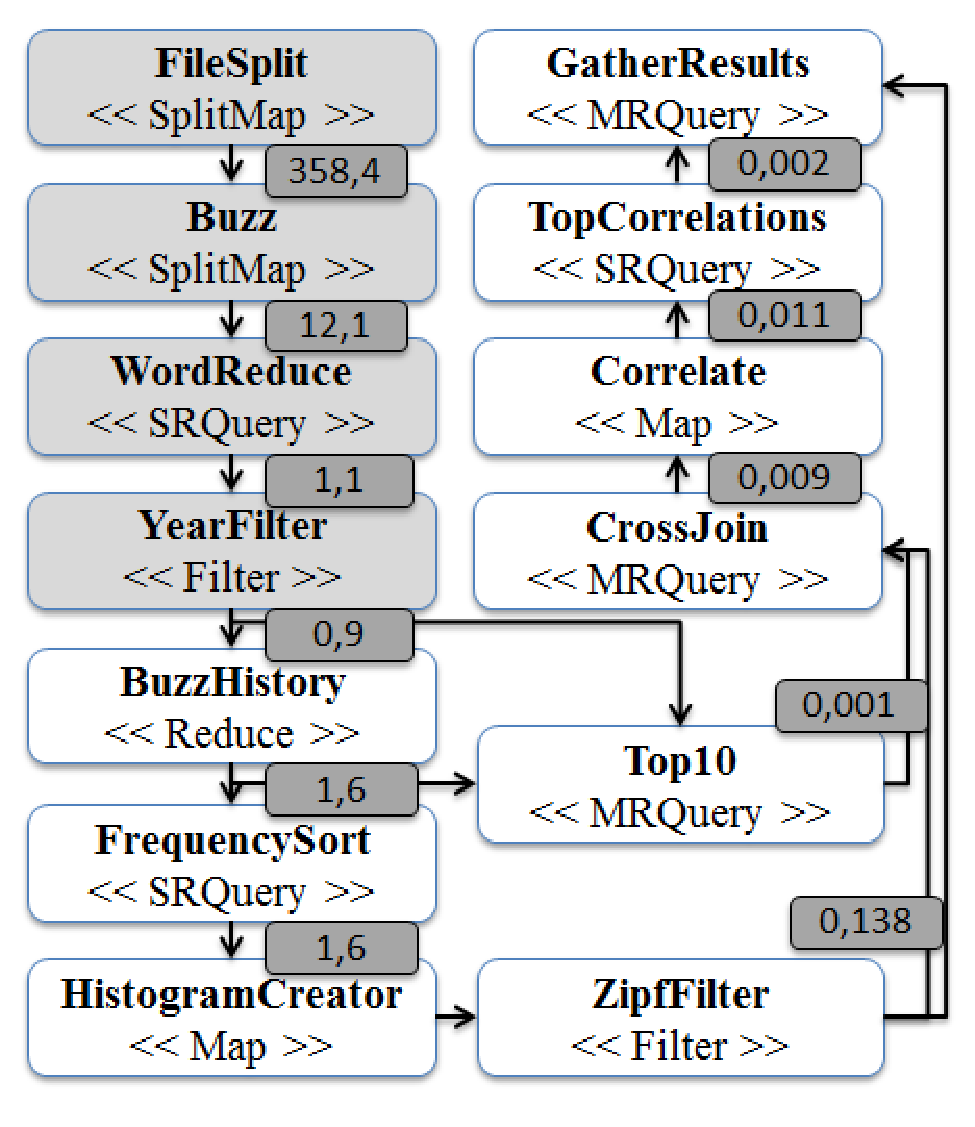
\includegraphics[width=2.3in]{figures/SF2} \label{fig:f1-2}}
		\subfigure[\textbf{Computing capacity adaptation technique.}]{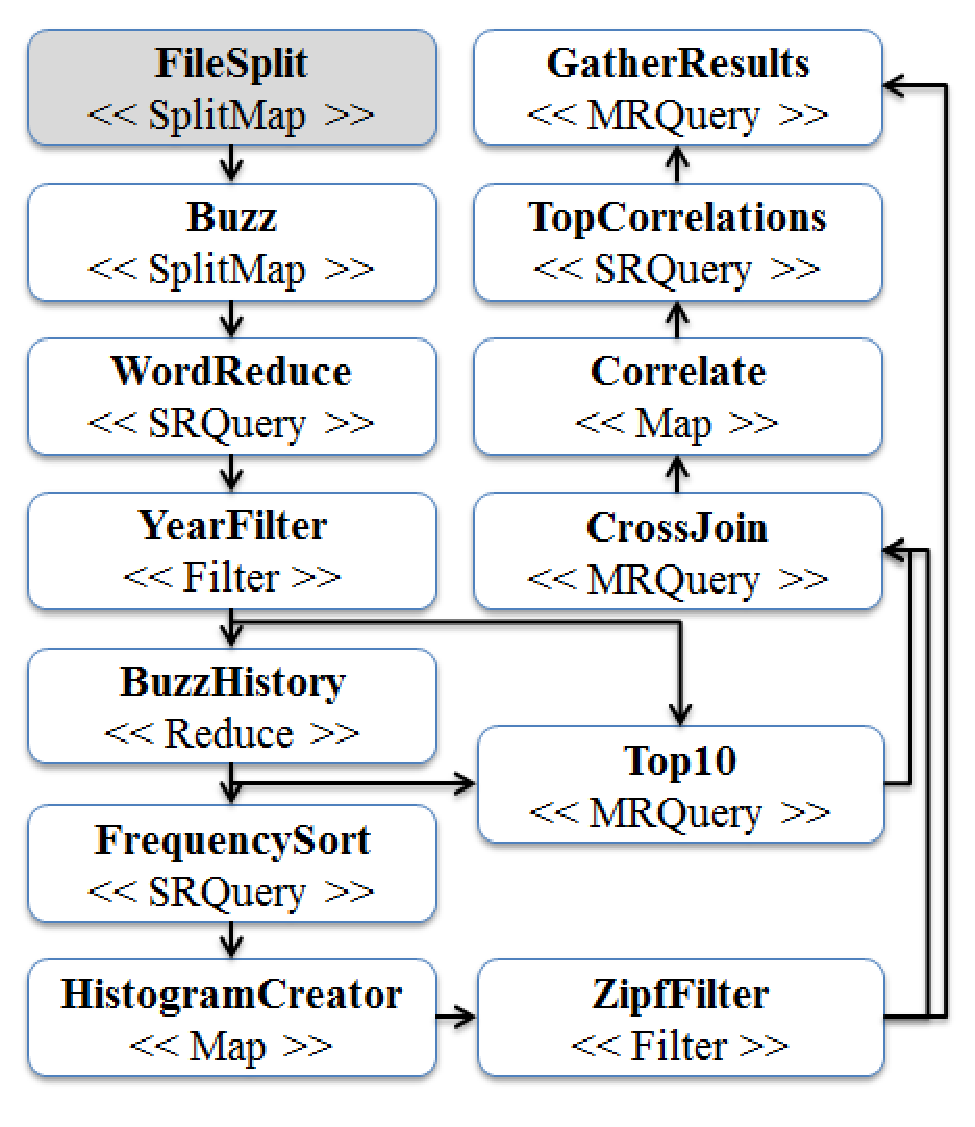
\includegraphics[width=2.3in]{figures/SF3} \label{fig:f1-3}} \\
		\subfigure{
\includegraphics[width=4.6in]{figures/SF5}}\\
	\end{centering}
\caption{\textbf{Buzz SWf partitioning. }}
\label{fig:f1} 
\end{figure}

In the remainder of the chapter, we assume that there are two cloud sites (\textit{$S_{1}$} and \textit{$S_{2}$}) to execute Buzz SWf.
A fixed activity is located at a specific site and cannot be moved to another site because of additional restrictions, 
\textit{i.e.} scientist security, data transfer, computing capacity and proprietary issues.
We also assume that the first activity (\textit{FileSplit}) is a fixed activity at \textit{$S_{1}$} since the input data located at \textit{$S_{1}$} is very big. 
In addition, we assume that the last activity (\textit{GatherResults}) is a fixed activity at \textit{$S_{2}$} because of proprietary issues. 
Finally, scientists at \textit{$S_{2}$} need to monitor the execution of activity \textit{HistogramCreator} without malicious attack
and thus, \textit{HistogramCreator} becomes a fixed activity at \textit{$S_{2}$}, which is trusted by scientists.

\section{Workflow Partitioning Techniques}
\label{sec:WPT}

In this section, we present the approaches to partition a SWf into fragments.
SWf partitioning is the process of dividing a SWf and input data into several fragments, so that each fragment can be executed at a site. It can be performed by DAG partitioning or data partitioning. DAG partitioning transforms a DAG composed of activities into a DAG composed of fragments while each fragment is a DAG composed of activities and dependencies. Data partitioning divides the input data of a fragment generated by DAG partitioning into several data sets, each of which is encapsulated in a newly generated fragment. This chapter focuses on the DAG partitioning.

The smallest granularity of fragment is an activity. Thus, we can encapsulate each activity in one fragment. 
We call this method activity encapsulation partitioning. 
However, this method is very simple and not optimized for the execution environment. 
In this chapter, we propose to partition the SWf according to the structure of the SWf or the execution environment.
We propose three techniques for SWf partitioning, \textit{i.e.} scientist privacy, 
data transfer minimization and computing capacity adaptation. 

The first technique, Scientist Privacy (SPr), is for better supporting SWf activity monitoring under scientist security restriction. 
When a SWf contains an activity that needs to be monitored by scientists, this activity is defined as a locking activity to be executed at a trusted cloud site to avoid malicious attack during SWf execution. 
A locking activity implies that this activity and all the following activities should be assigned to a same fragment, 
in order to provide further activity monitoring. 
The following activities represent the activities that process the output data or the data produced from the output data of the locking activity.
In order to partition a SWf based on scientist privacy technique, 
a SWfMS identifies the locking activity. 
Then it can partition the SWf by putting the locking activity and its available following activities (the following activities that are not fixed activities) into a fragment. 
According to this technique, Buzz SWf is partitioned into two fragments as shown in Fig. \ref{fig:f1-1}. 
As scientists need to analyze some histogram files produced by \textit{HistogramCreator} activity at runtime at \textit{$S_{2}$} (trusted by scientists),  
\textit{HistogramCreator} activity is handled as a locking activity.
This activity and the following activities (\textit{ZipfFilter}, \textit{CrossJoin}, \textit{Correlate}, \textit{TopCorrelations} and \textit{GatherResults}) are assigned to the same fragment while the other activities stay in another fragment.

The second technique is Data Transfer Minimization (DTM), which minimizes the volume of data to be transferred between different fragments. It is based on the fact that it takes much time to transfer certain amount of data from one site to another site. If the amount of data to be transferred between fragments is minimized, the time to transfer data between different sites can be reduced so as to reduce the entire execution time. During SWf design, the ratio between the volume of input data and output data can be offered. The scientists can estimate the data transfer for each data dependency based on the volume of input data of the SWf. The corresponding algorithm is shown in Algorithm \ref{alg:wp}.

\linespread{1.0}
\begin{algorithm}[ht]
\caption{Data transfer minimization SWf partitioning}\label{alg:wp}
\begin{algorithmic}[1]
\INPUT $SWf$: a SWf;
$S$: a set of sites
\OUTPUT $DS$: a set of dependencies to cut in order to partition the SWf
\BEGIN
\State $DS\gets \emptyset$
\ForAll{$s \in S$}
\State $A\gets$ fixedActvities$( SWf, s )$
\State $A’\gets$ fixedOutsideUnprocessedActivities$( SWf, s )$
\ForAll{$a \in A$}
\ForAll{$a' \in A'$}
\State $paths\gets$ findPaths$( a, a’ )$
\ForAll{$path \in paths$}
\State $ds\gets$ minData$(path)$
\State $DS\gets DS \bigcup ds$
\EndFor
\EndFor
\EndFor
\EndFor
\State $DS\gets sort(DS)$ 
\ForAll{$ds\in DS$}
\If{$SWf$ can be partitioned by $DS$ without $ds$)}
\State $DS\gets DS - ds $
\EndIf
\EndFor
\ENDBEGIN
\end{algorithmic}
\end{algorithm}

In Algorithm \ref{alg:wp}, a set of data dependencies $DS$ are chosen to be removed from the original SWf in order to partition the SWf. In this algorithm, the input data is viewed as a fixed activity. Lines $2-10$ select the dependencies to be removed in order to partition the activities of the SWf at each site. Line $4$ selects the fixed activities that are outside of Site $s$ and that the corresponding sites are not processed. If one site is processed in the loop of Lines $5-11$, it is marked as processed. For the two functions $fixedActivities$ and $fixedOutsideUnprocessedActivities$, each activity is checked to know if the activity is to be selected. Lines $7 - 10$ choose the dependencies to be removed so that the fixed activities at Site $s$ are not connected with the fixed activities at other sites. 
Line $7$ finds all the paths that connect two activities fixed at different sites. A path has a set of data dependencies that can connect two activities without consideration of direction. 
In order to find all the paths, a depth-first search algorithm can be used. For each path (Line $8$), the data dependency that has the least amount of data to be transferred is selected (Line $9$) to $DS$ (Line $10$).  
At the same time, the input activity and output activity of the selected data dependency are marked.
Line $11$ sorts the data dependencies according to the amount of data to be transferred in descending order. If two or more data dependencies have the same amount of data, they are sorted according to the amount of output data of the following activity of each data dependency in descending order. This order allows the activities that have bigger data dependencies with their following activities to be connected with their following activities, after the removing of dependencies (Lines $12-14$), in order to reduce the amount of data to be transferred among different fragments. Lines $12-14$ remove data dependencies from $DS$ while ensuring that the SWf can always be partitioned with $DS$. Checking if SWf can be partitioned by a set of dependencies can be realized by checking if the corresponding input and output activities of $ds$ are connected with a depth-first search algorithm (Line $13$).

With this algorithm, Buzz SWf is partitioned as shown in Fig. \ref{fig:f1-2}. 
The dark gray boxes represent the data transfer volume for the corresponding dependencies.
The data dependencies of each possible route between \textit{FileSplit} and \textit{HistogramCreator} is analyzed. 
The dependencies (\textit{YearFilter} to \textit{BuzzHistory} and \textit{YearFilter} to \textit{Top10}) are put in $DS$ to be removed.
Finally, Buzz SWf is partitioned by removing the selected dependencies (\textit{YearFilter} to \textit{BuzzHistory} and \textit{YearFilter} to \textit{Top10}).


The third technique is Computing Capacity Adaptation (CCA), which adapts SWfs partitioning to the computing capacity at different cloud sites. 
This technique is for the heterogeneous multisite cloud configurations, which may be incurred by the different configurations of different groups of scientists.
If a SWf is partitioned into two fragments that are sequentially executed, 
\textit{i.e.} one fragment begins execution after the execution of another one,
a SWfMS can put all the possible activities to one fragment while leaving fixed activities in another fragment. 
As an example, Buzz SWf is partitioned into two fragments (\textit{$WF_{1}$} and \textit{$WF_{2}$}) as shown in Fig. \ref{fig:f1-3} . 
Since the input data of activity \textit{FileSplit} is relatively big and located at a specific site, we keep this activity in the gray fragment.
Then, the white fragments can be scheduled to a cloud site that has more computing capacity.



\section{Validation}
\label{sec:SWEMCVal}

In this section, we present experiments to validate our approach, by executing
Buzz SWf using our partitioning techniques in Microsoft Azure cloud. 
The VMs are distributed at two cloud sites: Western Europe (Amsterdam, Netherlands) and Eastern US (North Virginia). 
In the first experiment,
we use a homogeneous configuration by creating two A$4$ VMs at both of Western Europe site and Eastern US site.
In the second experiment,
we use a heterogeneous configuration by creating two A$4$ VMs at the Western Europe site and eight A$4$ VMs
at the Eastern US site. 
Each A$4$ VM has $8$ CPU cores, $14$ GB of RAM memory, $127$ GB of instance storage and a network of $800$ Mbps \cite{VMA,VMB}. 

We executed Buzz SWf with Chiron and the SWf partitioner.
We used Linux \textit{tar} command and Linux \textit{scp} command for data refining and data transfer.
We launched the fragment execution by hand at each cloud site, which resembles to the cooperation between two scientist group.
In our execution, Chiron exploits data parallelism and the dynamic scheduling method for SWf parallel execution within one site.
Table \ref{tab:sim-1} shows the experimental results. 
Elapsed time $1$ represents the execution time without considering data transfer time. 
Elapsed time $2$ shows the execution time plus the data transfer time. 
Elapsed time $3$ is the execution time plus data transfer time with data refining. 
Data transfer $1$ reveals the data transfer time without data refining. 
Data transfer $2$ presents the data refining and data transfer time. 
The three techniques correspond to the three partitioning techniques as explained in Section $5$.

\begin{table}
\caption{\textbf{Experimental Results.}}
\label{tab:sim-1}
\begin{centering}
\begin{tabular}{|c|c|c|c|c|c|}
\hline 
Approach & Execution & Transmission & Execution & Transmission & Execution \tabularnewline
(Time in minutes) & time 1 & time 1 & time 2 & time 2 & time 3 \tabularnewline

\hline 
$1^{st}$ experiment & \multicolumn{5}{c|}{2*A4 VM (EU) + 2*A4 VM (US)} \tabularnewline
\hline
SPr technique & $199$ & $38$ & $237$ & $0$ & $199$ \tabularnewline
DTM technique & $186$ & $0$ & $186$ & $0$ & $186$ \tabularnewline
CCA technique & $209$ & $35$ & $245$ & $0.5$ & $209$ \tabularnewline
\hline 
$1^{st}$ experiment & \multicolumn{5}{c|}{2*A4 VM (EU) + 8*A4 VM (US)} \tabularnewline
\hline
SPr technique & $198$ & $38$ & $236$ & $0$ & $198$ \tabularnewline
DTM technique & $182$ & $0$ & $182$ & $0$ & $182$ \tabularnewline
CCA technique & $169$ & $35$ & $201$ & $0.5$ & $169$ \tabularnewline
\hline 
\end{tabular}
\par\end{centering}
\end{table}

In the first experiment, the SWf execution time of the three techniques without considering data transfer time is different 
because there are different amounts of data loaded into RAM memory for the white SWf fragment execution. 
Since the DTM technique minimizes the data transfer between two fragments, 
it also reduces the data to be transferred from disk to RAM at the beginning of the second fragment (white fragment) execution.
When the data is transferred without data refining, the execution time of the DTM technique is $21.5\%$ and $24.1\%$ less than the SPr and the CCA technique.
When the data is transferred with data refining, the DTM technique saves $6.5\%$ and $11.0\%$ of the execution time compared to the SPr and the CCA technique.
As the two sites have the same computing capacity and it incurs big data transfer volume, the CCA is the least efficient technique.
In this experiment, the SWf execution with the best partitioning technique (DTM with data refining) takes $24.1\%$ less time than the least efficient technique (CCA without data refining).
In the second experiment, because of the difference of computing capacity at two cloud sites, 
the execution of the CCA technique takes the least amount of time without considering data transfer. 
When the data is transferred without data refining, 
the DTM technique is still the best performance because of the minimized data transfer cost. 
This technique yields a gain of $22.9\%$ and $10.4\%$ of the execution time compared to the SPr and CCA technique.
However, when we use data refining techniques, 
the third technique yields the best performance because of the adaptation of SWf partitioning to the computing capacity at each cloud site.
In this case, the SWf execution of the CCA technique takes $14.6\%$ and $7.1\%$ less time compared to the SPr and DTM technique.
In this experiment, the best partitioning technique (CCA with data refining) saves $28.4\%$ time compared to the least efficient technique (SPr without data refining).

The experiments reveal that the DTM technique with data refining is the best for a homogeneous configuration 
and that the CCA technique with data refining has better performance for a heterogeneous configuration.

\section{Conclusion}
\label{sec:SWEMCCon}

The cloud is emerging as an appropriate infrastructure for SWf execution. 
However, because of different restrictions, a SWf often
needs to be partitioned and executed in parallel in a multisite
environment.
In this chapter, we proposed a non-intrusive approach to execute SWfs in a multisite cloud with three SWf partitioning
techniques.
We proposed a system model based on Chiron SWfMS and its adaptation to
multisite cloud and a SWf partitioner.
We presented the scheduling of fragment execution by respecting all the data dependencies in the original SWf. 
We described an experimental validation using an adaptation of Chiron
SWfMS for Microsoft Azure multisite cloud.
The experiments experiments reveal the efficiency of our partitioning
techniques, and their superiority in different environments.
The experiment results show that data transfer minimization technique with data refining, \textit{i.e.} file archiving and data compression, has better performance ($24.1\%$ of time saved compared to computing capacity adaptation technique without data refining) for homogeneous configurations
while computing capacity adaptation technique with data refining ($28.4\%$ of time saved compared to scientist privacy technique without data refining) is appropriate to heterogeneous configurations. 
